%%%%%%%%%%%%%%%%%%%%%%%%%%%%%%%%%%%%%%%%%%%%%%%%%%%%%%%%%%%%%%%%%%%%%%%%%%%%%%%%
% CHAPTER 2
%%%%%%%%%%%%%%%%%%%%%%%%%%%%%%%%%%%%%%%%%%%%%%%%%%%%%%%%%%%%%%%%%%%%%%%%%%%%%%%%

\chapter{Systems and Their Properties}

\begin{tcolorbox}[colback=blue!5!white,colframe=blue!70!black,title=Learning Objectives]

After studying this chapter, the reader will be able to

\begin{itemize}
\item Define a system and identify its input and output.
\item Distinguish between continuous-time and discrete-time systems.
\item Determine whether a system is linear or nonlinear.
\item Test time invariance of a system.
\item Check causality and memory properties.
\item Determine stability using the bounded-input bounded-output criterion.
\item Classify systems as static or dynamic.
\end{itemize}

\end{tcolorbox}

%%%%%%%%%%%%%%%%%%%%%%%%%%%%%%%%%%%%%%%%%%%%%%%%%%%%%%%%%%%%%%%%%%%%%%%%%%%%%%%%

\section{Introduction}

A signal by itself only carries information. A \textbf{system} is an entity that
processes the signal and produces another signal.

Examples include

\begin{itemize}
\item an amplifier,
\item a filter,
\item an analog-to-digital converter,
\item a communication channel,
\item a microcontroller,
\item and a digital signal-processing algorithm.
\end{itemize}

The study of system properties helps us predict how a system behaves for
different inputs and is essential for designing communication and control
systems.

%%%%%%%%%%%%%%%%%%%%%%%%%%%%%%%%%%%%%%%%%%%%%%%%%%%%%%%%%%%%%%%%%%%%%%%%%%%%%%%%

\section{What is a System?}

\subsection{Definition}

A \textbf{system} is a mathematical operation that transforms an input signal
into an output signal.

\[
\boxed{
y(t)=T\{x(t)\}
}
\]

or, for discrete time,

\[
\boxed{
y[n]=T\{x[n]\}
}
\]

where

\begin{itemize}
\item \(x\): input signal,
\item \(y\): output signal,
\item \(T\): system operator.
\end{itemize}

%%%%%%%%%%%%%%%%%%%%%%%%%%%%%%%%%%%%%%%%%%%%%%%%%%%%%%%%%%%%%%%%%%%%%%%%%%%%%%%%

\section{Block Representation}

\begin{center}
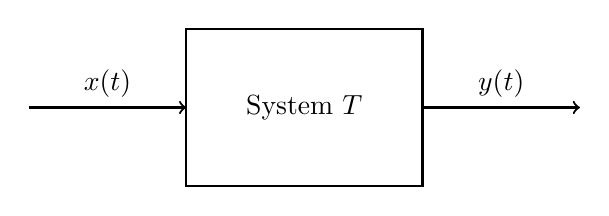
\begin{tikzpicture}[scale=1]
\draw[->,thick] (-3,0) -- (-1,0) node[midway,above] {$x(t)$};
\draw[thick] (-1,-1) rectangle (2,1);
\node at (0.5,0) {System $T$};
\draw[->,thick] (2,0) -- (4,0) node[midway,above] {$y(t)$};
\end{tikzpicture}
\end{center}

The system receives \(x(t)\) and produces \(y(t)\).

%%%%%%%%%%%%%%%%%%%%%%%%%%%%%%%%%%%%%%%%%%%%%%%%%%%%%%%%%%%%%%%%%%%%%%%%%%%%%%%%

\section{Continuous-Time and Discrete-Time Systems}

%%%%%%%%%%%%%%%%%%%%%%%%%%%%%%%%%%%%%%%%%%%%%%%%%%%%%%%%%%%%%%%%%%%%%%%%%%%%%%%%

\subsection{Continuous-Time System}

Input and output are continuous-time signals.

Example:

\[
y(t)=2x(t)+5
\]

%%%%%%%%%%%%%%%%%%%%%%%%%%%%%%%%%%%%%%%%%%%%%%%%%%%%%%%%%%%%%%%%%%%%%%%%%%%%%%%%

\subsection{Discrete-Time System}

Input and output are discrete-time signals.

Example:

\[
y[n]=x[n]+x[n-1]
\]

%%%%%%%%%%%%%%%%%%%%%%%%%%%%%%%%%%%%%%%%%%%%%%%%%%%%%%%%%%%%%%%%%%%%%%%%%%%%%%%%

\section{Memoryless and Dynamic Systems}

%%%%%%%%%%%%%%%%%%%%%%%%%%%%%%%%%%%%%%%%%%%%%%%%%%%%%%%%%%%%%%%%%%%%%%%%%%%%%%%%

\subsection{Memoryless System}

A system is memoryless if the output at time \(t\) depends only on the input at
the same time \(t\).

\[
\boxed{
y(t)=f(x(t))
}
\]

Example:

\[
y(t)=3x(t)
\]

This system is memoryless.

%%%%%%%%%%%%%%%%%%%%%%%%%%%%%%%%%%%%%%%%%%%%%%%%%%%%%%%%%%%%%%%%%%%%%%%%%%%%%%%%

\subsection{Dynamic System}

A system has memory if the output depends on past or future values of the input.

Example:

\[
y(t)=x(t)+x(t-1)
\]

Since \(x(t-1)\) is involved, the system is dynamic.

%%%%%%%%%%%%%%%%%%%%%%%%%%%%%%%%%%%%%%%%%%%%%%%%%%%%%%%%%%%%%%%%%%%%%%%%%%%%%%%%

\section{Linear and Nonlinear Systems}

%%%%%%%%%%%%%%%%%%%%%%%%%%%%%%%%%%%%%%%%%%%%%%%%%%%%%%%%%%%%%%%%%%%%%%%%%%%%%%%%

\subsection{Linearity Conditions}

A system is linear if it satisfies

\begin{enumerate}
\item \textbf{Additivity}
\item \textbf{Homogeneity (scaling)}
\end{enumerate}

%%%%%%%%%%%%%%%%%%%%%%%%%%%%%%%%%%%%%%%%%%%%%%%%%%%%%%%%%%%%%%%%%%%%%%%%%%%%%%%%

\subsection{Additivity}

If

\[
T\{x_1(t)\}=y_1(t)
\]

\[
T\{x_2(t)\}=y_2(t),
\]

then

\[
\boxed{
T\{x_1(t)+x_2(t)\}=y_1(t)+y_2(t)
}
\]

%%%%%%%%%%%%%%%%%%%%%%%%%%%%%%%%%%%%%%%%%%%%%%%%%%%%%%%%%%%%%%%%%%%%%%%%%%%%%%%%

\subsection{Homogeneity}

For any constant \(a\),

\[
\boxed{
T\{ax(t)\}=aT\{x(t)\}
}
\]

%%%%%%%%%%%%%%%%%%%%%%%%%%%%%%%%%%%%%%%%%%%%%%%%%%%%%%%%%%%%%%%%%%%%%%%%%%%%%%%%

\subsection{Superposition}

Combining both conditions,

\[
\boxed{
T\{a_1x_1(t)+a_2x_2(t)\}
=
a_1y_1(t)+a_2y_2(t)
}
\]

This is the superposition principle.

%%%%%%%%%%%%%%%%%%%%%%%%%%%%%%%%%%%%%%%%%%%%%%%%%%%%%%%%%%%%%%%%%%%%%%%%%%%%%%%%

\section{Example: Linear System}

Consider

\[
y(t)=2x(t).
\]

For input \(ax_1(t)+bx_2(t)\),

\[
T\{ax_1+bx_2\}
=
2(ax_1+bx_2)
\]

\[
=2ax_1+2bx_2
\]

\[
=a(2x_1)+b(2x_2)
\]

\[
=aT\{x_1\}+bT\{x_2\}.
\]

Hence,

\[
\boxed{
y(t)=2x(t)\ \text{is linear}
}
\]

%%%%%%%%%%%%%%%%%%%%%%%%%%%%%%%%%%%%%%%%%%%%%%%%%%%%%%%%%%%%%%%%%%%%%%%%%%%%%%%%

\section{Example: Nonlinear System}

Consider

\[
y(t)=x^2(t).
\]

For input \(ax(t)\),

\[
T\{ax(t)\}=(ax(t))^2=a^2x^2(t).
\]

But

\[
aT\{x(t)\}=ax^2(t).
\]

Since

\[
a^2x^2(t)\neq ax^2(t),
\]

the homogeneity condition fails.

Therefore,

\[
\boxed{
y(t)=x^2(t)\ \text{is nonlinear}
}
\]

%%%%%%%%%%%%%%%%%%%%%%%%%%%%%%%%%%%%%%%%%%%%%%%%%%%%%%%%%%%%%%%%%%%%%%%%%%%%%%%%

\section{Time-Invariant Systems}

%%%%%%%%%%%%%%%%%%%%%%%%%%%%%%%%%%%%%%%%%%%%%%%%%%%%%%%%%%%%%%%%%%%%%%%%%%%%%%%%

\subsection{Definition}

A system is time invariant if a delay in the input produces the same delay in
the output.

%%%%%%%%%%%%%%%%%%%%%%%%%%%%%%%%%%%%%%%%%%%%%%%%%%%%%%%%%%%%%%%%%%%%%%%%%%%%%%%%

\subsection{Test Procedure}

Suppose

\[
T\{x(t)\}=y(t).
\]

Delay the input:

\[
x_d(t)=x(t-t_0).
\]

Compute the system output:

\[
T\{x(t-t_0)\}.
\]

Now delay the original output:

\[
y(t-t_0).
\]

If

\[
\boxed{
T\{x(t-t_0)\}=y(t-t_0)
}
\]

the system is time invariant.

%%%%%%%%%%%%%%%%%%%%%%%%%%%%%%%%%%%%%%%%%%%%%%%%%%%%%%%%%%%%%%%%%%%%%%%%%%%%%%%%

\section{Example: Time-Invariant System}

Consider

\[
y(t)=x(t)+x(t-1).
\]

For delayed input,

\[
T\{x(t-t_0)\}
=
x(t-t_0)+x(t-t_0-1).
\]

The delayed output is

\[
y(t-t_0)
=
x(t-t_0)+x(t-t_0-1).
\]

Both are identical.

Hence,

\[
\boxed{
y(t)=x(t)+x(t-1)\ \text{is time invariant}
}
\]

%%%%%%%%%%%%%%%%%%%%%%%%%%%%%%%%%%%%%%%%%%%%%%%%%%%%%%%%%%%%%%%%%%%%%%%%%%%%%%%%

\section{Example: Time-Varying System}

Consider

\[
y(t)=tx(t).
\]

For delayed input,

\[
T\{x(t-t_0)\}=t\,x(t-t_0).
\]

Delayed output:

\[
y(t-t_0)=(t-t_0)x(t-t_0).
\]

Since these are not equal,

\[
\boxed{
y(t)=tx(t)\ \text{is time varying}
}
\]

%%%%%%%%%%%%%%%%%%%%%%%%%%%%%%%%%%%%%%%%%%%%%%%%%%%%%%%%%%%%%%%%%%%%%%%%%%%%%%%%

\section{Quick Identification Table}

\begin{table}[H]
\centering
\caption{Quick classification}
\begin{tabular}{|p{5cm}|p{5cm}|}
\hline
\textbf{System} & \textbf{Classification} \\
\hline
\(y(t)=3x(t)\) & Linear, memoryless, TI \\
\hline
\(y(t)=x^2(t)\) & Nonlinear \\
\hline
\(y(t)=x(t-1)\) & Linear, dynamic, TI \\
\hline
\(y(t)=tx(t)\) & Linear, time varying \\
\hline
\(y(t)=x(t)+5\) & Nonlinear (fails homogeneity) \\
\hline
\end{tabular}
\end{table}

%%%%%%%%%%%%%%%%%%%%%%%%%%%%%%%%%%%%%%%%%%%%%%%%%%%%%%%%%%%%%%%%%%%%%%%%%%%%%%%%

\begin{tcolorbox}[title=Quick Recall,colback=yellow!10]

\[
y(t)=T\{x(t)\}
\]

\[
T\{a_1x_1+a_2x_2\}=a_1T\{x_1\}+a_2T\{x_2\}
\]

\[
T\{x(t-t_0)\}=y(t-t_0)
\]

Memoryless: depends only on \(x(t)\)

Dynamic: depends on \(x(t\pm\tau)\)

\end{tcolorbox}
%%%%%%%%%%%%%%%%%%%%%%%%%%%%%%%%%%%%%%%%%%%%%%%%%%%%%%%%%%%%%%%%%%%%%%%%%%%%%%%%
%%%%%%%%%%%%%%%%%%%%%%%%%%%%%%%%%%%%%%%%%%%%%%%%%%%%%%%%%%%%%%%%%%%%%%%%%%%%%%%%
\section{Causal and Noncausal Systems}

%%%%%%%%%%%%%%%%%%%%%%%%%%%%%%%%%%%%%%%%%%%%%%%%%%%%%%%%%%%%%%%%%%%%%%%%%%%%%%%%

\subsection{Definition of Causality}

A system is \textbf{causal} if the output at time \(t\) depends only on

\begin{itemize}
\item present input values,
\item and past input values.
\end{itemize}

Mathematically, a causal system cannot depend on \(x(t+\tau)\) where
\(\tau>0\).

%%%%%%%%%%%%%%%%%%%%%%%%%%%%%%%%%%%%%%%%%%%%%%%%%%%%%%%%%%%%%%%%%%%%%%%%%%%%%%%%

\subsection{Examples of Causal Systems}

\[
y(t)=x(t)
\]

\[
y(t)=x(t-2)
\]

\[
y(t)=x(t)+x(t-1)
\]

These systems use only present or past values of the input.

%%%%%%%%%%%%%%%%%%%%%%%%%%%%%%%%%%%%%%%%%%%%%%%%%%%%%%%%%%%%%%%%%%%%%%%%%%%%%%%%

\subsection{Example of a Noncausal System}

\[
y(t)=x(t+1)
\]

Here, the output at time \(t\) depends on the future value of the input.

Therefore,

\[
\boxed{
y(t)=x(t+1)\ \text{is noncausal}
}
\]

%%%%%%%%%%%%%%%%%%%%%%%%%%%%%%%%%%%%%%%%%%%%%%%%%%%%%%%%%%%%%%%%%%%%%%%%%%%%%%%%

\section{Causality Test}

For a system described by

\[
y(t)=f(x(t),x(t-1),x(t+1),\ldots),
\]

\begin{itemize}
\item if only \(x(t)\) and \(x(t-\tau)\) appear, the system is causal;
\item if any \(x(t+\tau)\) appears, the system is noncausal.
\end{itemize}

%%%%%%%%%%%%%%%%%%%%%%%%%%%%%%%%%%%%%%%%%%%%%%%%%%%%%%%%%%%%%%%%%%%%%%%%%%%%%%%%

\section{Stability}

%%%%%%%%%%%%%%%%%%%%%%%%%%%%%%%%%%%%%%%%%%%%%%%%%%%%%%%%%%%%%%%%%%%%%%%%%%%%%%%%

\subsection{BIBO Stability}

A system is \textbf{bounded-input bounded-output (BIBO) stable} if every bounded
input produces a bounded output.

If

\[
|x(t)|\le M_x<\infty,
\]

then there must exist a finite constant \(M_y\) such that

\[
|y(t)|\le M_y<\infty.
\]

%%%%%%%%%%%%%%%%%%%%%%%%%%%%%%%%%%%%%%%%%%%%%%%%%%%%%%%%%%%%%%%%%%%%%%%%%%%%%%%%

\section{Example: Stable System}

Consider

\[
y(t)=0.5\,x(t).
\]

If

\[
|x(t)|\le M,
\]

then

\[
|y(t)|=0.5|x(t)|\le 0.5M.
\]

Since \(0.5M\) is finite,

\[
\boxed{
y(t)=0.5x(t)\ \text{is stable}
}
\]

%%%%%%%%%%%%%%%%%%%%%%%%%%%%%%%%%%%%%%%%%%%%%%%%%%%%%%%%%%%%%%%%%%%%%%%%%%%%%%%%

\section{Example: Unstable System}

Consider

\[
y(t)=t\,x(t).
\]

Choose a bounded input

\[
x(t)=1.
\]

Then

\[
y(t)=t.
\]

As \(t\to\infty\),

\[
|y(t)|\to\infty.
\]

Hence,

\[
\boxed{
y(t)=t\,x(t)\ \text{is unstable}
}
\]

%%%%%%%%%%%%%%%%%%%%%%%%%%%%%%%%%%%%%%%%%%%%%%%%%%%%%%%%%%%%%%%%%%%%%%%%%%%%%%%%

\section{Stability of LTI Systems}

For a continuous-time LTI system with impulse response \(h(t)\),

\[
\boxed{
\int_{-\infty}^{\infty}|h(t)|\,dt<\infty
}
\]

is the condition for BIBO stability.

For a discrete-time LTI system,

\[
\boxed{
\sum_{n=-\infty}^{\infty}|h[n]|<\infty
}
\]

%%%%%%%%%%%%%%%%%%%%%%%%%%%%%%%%%%%%%%%%%%%%%%%%%%%%%%%%%%%%%%%%%%%%%%%%%%%%%%%%

\section{Example Using Impulse Response}

Suppose

\[
h(t)=e^{-t}u(t).
\]

Then,

\[
\int_{-\infty}^{\infty}|h(t)|dt
=
\int_0^\infty e^{-t}dt
\]

\[
=
\left[-e^{-t}\right]_0^\infty
=1.
\]

Since the integral is finite,

\[
\boxed{
h(t)=e^{-t}u(t)\ \text{is stable}
}
\]

%%%%%%%%%%%%%%%%%%%%%%%%%%%%%%%%%%%%%%%%%%%%%%%%%%%%%%%%%%%%%%%%%%%%%%%%%%%%%%%%

\section{Invertible Systems}

%%%%%%%%%%%%%%%%%%%%%%%%%%%%%%%%%%%%%%%%%%%%%%%%%%%%%%%%%%%%%%%%%%%%%%%%%%%%%%%%

\subsection{Definition}

A system is \textbf{invertible} if different inputs produce different outputs
and the original input can be uniquely recovered from the output.

%%%%%%%%%%%%%%%%%%%%%%%%%%%%%%%%%%%%%%%%%%%%%%%%%%%%%%%%%%%%%%%%%%%%%%%%%%%%%%%%

\subsection{Example: Invertible}

\[
y(t)=2x(t).
\]

The inverse system is

\[
x(t)=\frac{y(t)}{2}.
\]

Hence,

\[
\boxed{
y(t)=2x(t)\ \text{is invertible}
}
\]

%%%%%%%%%%%%%%%%%%%%%%%%%%%%%%%%%%%%%%%%%%%%%%%%%%%%%%%%%%%%%%%%%%%%%%%%%%%%%%%%

\subsection{Example: Noninvertible}

\[
y(t)=x^2(t).
\]

If

\[
x_1(t)=1,\qquad x_2(t)=-1,
\]

both produce

\[
y(t)=1.
\]

Since the input cannot be uniquely determined,

\[
\boxed{
y(t)=x^2(t)\ \text{is noninvertible}
}
\]

%%%%%%%%%%%%%%%%%%%%%%%%%%%%%%%%%%%%%%%%%%%%%%%%%%%%%%%%%%%%%%%%%%%%%%%%%%%%%%%%

\section{Static and Dynamic Systems}

%%%%%%%%%%%%%%%%%%%%%%%%%%%%%%%%%%%%%%%%%%%%%%%%%%%%%%%%%%%%%%%%%%%%%%%%%%%%%%%%

\subsection{Static (Memoryless)}

\[
y(t)=f(x(t))
\]

Example:

\[
y(t)=5x(t).
\]

%%%%%%%%%%%%%%%%%%%%%%%%%%%%%%%%%%%%%%%%%%%%%%%%%%%%%%%%%%%%%%%%%%%%%%%%%%%%%%%%

\subsection{Dynamic (With Memory)}

\[
y(t)=f(x(t),x(t-\tau),x(t+\tau),\ldots)
\]

Example:

\[
y(t)=x(t)+x(t-1).
\]

%%%%%%%%%%%%%%%%%%%%%%%%%%%%%%%%%%%%%%%%%%%%%%%%%%%%%%%%%%%%%%%%%%%%%%%%%%%%%%%%

\section{Complete Classification Procedure}

Given a system:

\[
y(t)=f(x(t),x(t\pm\tau),t),
\]

use the following sequence:

%%%%%%%%%%%%%%%%%%%%%%%%%%%%%%%%%%%%%%%%%%%%%%%%%%%%%%%%%%%%%%%%%%%%%%%%%%%%%%%%

\subsection{Step 1: Memory}

\begin{itemize}
\item only \(x(t)\) \(\rightarrow\) memoryless,
\item delayed/advanced terms \(\rightarrow\) dynamic.
\end{itemize}

%%%%%%%%%%%%%%%%%%%%%%%%%%%%%%%%%%%%%%%%%%%%%%%%%%%%%%%%%%%%%%%%%%%%%%%%%%%%%%%%

\subsection{Step 2: Linearity}

Check superposition:

\[
T\{a_1x_1+a_2x_2\}
\stackrel{?}{=}
a_1T\{x_1\}+a_2T\{x_2\}.
\]

%%%%%%%%%%%%%%%%%%%%%%%%%%%%%%%%%%%%%%%%%%%%%%%%%%%%%%%%%%%%%%%%%%%%%%%%%%%%%%%%

\subsection{Step 3: Time Invariance}

Check

\[
T\{x(t-t_0)\}
\stackrel{?}{=}
y(t-t_0).
\]

%%%%%%%%%%%%%%%%%%%%%%%%%%%%%%%%%%%%%%%%%%%%%%%%%%%%%%%%%%%%%%%%%%%%%%%%%%%%%%%%

\subsection{Step 4: Causality}

Look for future terms \(x(t+\tau)\).

%%%%%%%%%%%%%%%%%%%%%%%%%%%%%%%%%%%%%%%%%%%%%%%%%%%%%%%%%%%%%%%%%%%%%%%%%%%%%%%%

\subsection{Step 5: Stability}

Apply the BIBO test.

%%%%%%%%%%%%%%%%%%%%%%%%%%%%%%%%%%%%%%%%%%%%%%%%%%%%%%%%%%%%%%%%%%%%%%%%%%%%%%%%

\subsection{Step 6: Invertibility}

Determine whether the input can be uniquely recovered.

%%%%%%%%%%%%%%%%%%%%%%%%%%%%%%%%%%%%%%%%%%%%%%%%%%%%%%%%%%%%%%%%%%%%%%%%%%%%%%%%

\section{Flowchart}

For quick classification of a system, follow this sequence:

\begin{enumerate}
\item Check whether the output depends only on the present input.
\item Check linearity using the superposition principle.
\item Check time invariance.
\item Check causality.
\item Check stability.
\item Check invertibility.
\end{enumerate}

This procedure is sufficient for solving most GATE and university examination problems.
%%%%%%%%%%%%%%%%%%%%%%%%%%%%%%%%%%%%%%%%%%%%%%%%%%%%%%%%%%%%%%%%%%%%%%%%%%%%%%%%

\section{Solved Classification Example}

Classify

\[
y(t)=x(t-1)+3x(t).
\]

%%%%%%%%%%%%%%%%%%%%%%%%%%%%%%%%%%%%%%%%%%%%%%%%%%%%%%%%%%%%%%%%%%%%%%%%%%%%%%%%

\subsection{Memory}

Depends on \(x(t-1)\) \(\Rightarrow\) dynamic.

%%%%%%%%%%%%%%%%%%%%%%%%%%%%%%%%%%%%%%%%%%%%%%%%%%%%%%%%%%%%%%%%%%%%%%%%%%%%%%%%

\subsection{Linearity}

Satisfies superposition \(\Rightarrow\) linear.

%%%%%%%%%%%%%%%%%%%%%%%%%%%%%%%%%%%%%%%%%%%%%%%%%%%%%%%%%%%%%%%%%%%%%%%%%%%%%%%%

\subsection{Time Invariance}

Delay property is preserved \(\Rightarrow\) time invariant.

%%%%%%%%%%%%%%%%%%%%%%%%%%%%%%%%%%%%%%%%%%%%%%%%%%%%%%%%%%%%%%%%%%%%%%%%%%%%%%%%

\subsection{Causality}

Only present and past values appear \(\Rightarrow\) causal.

%%%%%%%%%%%%%%%%%%%%%%%%%%%%%%%%%%%%%%%%%%%%%%%%%%%%%%%%%%%%%%%%%%%%%%%%%%%%%%%%

\subsection{Stability}

Bounded input gives bounded output \(\Rightarrow\) stable.

%%%%%%%%%%%%%%%%%%%%%%%%%%%%%%%%%%%%%%%%%%%%%%%%%%%%%%%%%%%%%%%%%%%%%%%%%%%%%%%%

\subsection{Final Classification}

\[
\boxed{
\text{Linear, Dynamic, Time-Invariant, Causal, Stable}
}
\]

%%%%%%%%%%%%%%%%%%%%%%%%%%%%%%%%%%%%%%%%%%%%%%%%%%%%%%%%%%%%%%%%%%%%%%%%%%%%%%%%

\section{Quick Classification Table}

\begin{table}[H]
\centering
\caption{Common systems and their properties}
\begin{tabular}{|p{5cm}|p{6cm}|}
\hline
\textbf{System} & \textbf{Properties} \\
\hline
\(y(t)=3x(t)\) & Linear, memoryless, TI, causal, stable \\
\hline
\(y(t)=x(t-2)\) & Linear, dynamic, TI, causal, stable \\
\hline
\(y(t)=x(t+2)\) & Linear, dynamic, TI, noncausal, stable \\
\hline
\(y(t)=tx(t)\) & Linear, memoryless, time varying, causal, unstable \\
\hline
\(y(t)=x^2(t)\) & Nonlinear, memoryless, TI, causal \\
\hline
\end{tabular}
\end{table}

%%%%%%%%%%%%%%%%%%%%%%%%%%%%%%%%%%%%%%%%%%%%%%%%%%%%%%%%%%%%%%%%%%%%%%%%%%%%%%%%

\section{Chapter Summary}

In this chapter, we introduced the concept of systems and studied their most
important properties:

\begin{itemize}
\item memoryless and dynamic,
\item linear and nonlinear,
\item time invariant and time varying,
\item causal and noncausal,
\item stable and unstable,
\item invertible and noninvertible.
\end{itemize}

These properties are fundamental for analyzing communication systems, filters,
control systems and digital signal-processing algorithms. In the next chapter,
we will study \textbf{Linear Time-Invariant (LTI) systems} and their impulse
response and convolution properties.

%%%%%%%%%%%%%%%%%%%%%%%%%%%%%%%%%%%%%%%%%%%%%%%%%%%%%%%%%%%%%%%%%%%%%%%%%%%%%%%%

\begin{tcolorbox}[title=One-Minute Revision,colback=blue!5]

\[
T\{a_1x_1+a_2x_2\}=a_1T\{x_1\}+a_2T\{x_2\}
\]

\[
T\{x(t-t_0)\}=y(t-t_0)
\]

Causal: no \(x(t+\tau)\)

Stable: bounded input \(\Rightarrow\) bounded output

Invertible: input can be uniquely recovered

LTI stability:

\[
\int_{-\infty}^{\infty}|h(t)|dt<\infty
\]

\[
\sum_{n=-\infty}^{\infty}|h[n]|<\infty
\]

\end{tcolorbox}
%%%%%%%%%%%%%%%%%%%%%%%%%%%%%%%%%%%%%%%%%%%%%%%%%%%%%%%%%%%%%%%%%%%%%%%%%%%%%%%%
